\documentclass{ieeeaccess}
\usepackage{cite}
\usepackage{amsmath,amssymb,amsfonts}
\usepackage{algorithmic}
\usepackage{graphicx}
\usepackage{textcomp}
\usepackage{booktabs}
\usepackage{array}
\usepackage{tabularx}
\usepackage{url}
\usepackage{bm}

\makeatletter
\AtBeginDocument{\DeclareMathVersion{bold}
\SetSymbolFont{operators}{bold}{T1}{times}{b}{n}
\SetSymbolFont{NewLetters}{bold}{T1}{times}{b}{it}
\SetMathAlphabet{\mathrm}{bold}{T1}{times}{b}{n}
\SetMathAlphabet{\mathit}{bold}{T1}{times}{b}{it}
\SetMathAlphabet{\mathbf}{bold}{T1}{times}{b}{n}
\SetMathAlphabet{\mathtt}{bold}{OT1}{pcr}{b}{n}
\SetSymbolFont{symbols}{bold}{OMS}{cmsy}{b}{n}
\renewcommand\boldmath{\@nomath\boldmath\mathversion{bold}}}
\makeatother

\def\BibTeX{{\rm B\kern-.05em{\sc i\kern-.025em b}\kern-.08em
    T\kern-.1667em\lower.7ex\hbox{E}\kern-.125emX}}

\begin{document}
\history{Date of publication August 00, 2026, date of current version August 00, 2026.}
\doi{10.1109/ACCESS.2026.0000000}

\title{From Statistical Evidence to Decision Value: Six Deployment Constraints on an Institutional Flow Dataset}

\author{\uppercase{Divyansh Singh}\authorrefmark{1},
\uppercase{Aryan Malviya}\authorrefmark{1},
\uppercase{Rishabh Masuriya}\authorrefmark{1},
\uppercase{and Pravin Patil}\authorrefmark{1}}
\address[1]{Department of Artificial Intelligence and Data Science, K.~J.~Somaiya Institute of Technology, Mumbai 400077, India (e-mail: divyansh26@somaiya.edu; aryan.malviya@somaiya.edu; rishabh.masuria@somaiya.edu; pravin.patil@somaiya.edu)}
\tfootnote{This research received no specific grant from any funding agency in the public, commercial, or not-for-profit sectors. Code and computational artifacts supporting this study are maintained under an open verification protocol.}

\markboth
{Singh \MakeLowercase{\textit{et al.}}: Six Deployment Constraints on an Institutional Flow Dataset}
{Singh \MakeLowercase{\textit{et al.}}: Six Deployment Constraints on an Institutional Flow Dataset}

\corresp{Corresponding author: Divyansh Singh (e-mail: divyansh26@somaiya.edu).}

\begin{abstract}
The replication literature in empirical asset pricing and quantitative finance has established that a majority of published return predictors fail conventional significance thresholds when re-tested. However, little is known regarding the trajectory of findings that do survive statistical re-examination once deployed under operational frictions. This study evaluates how far an alternative dataset carries once its statistical content is established, under the ordered constraints of production deployment. Using a fourteen-year transaction-level record of foreign institutional equity flows covering 25.15 million trades, we deploy the data across seven distinct points in a modeling stack: a cross-sectional volatility regression, a real-time filtered regime-switching model with a hazard layer, stock-day and market-level predictive density engines, a gradient-boosted feature attribution block, and a simulated long-short book. Each application faces six ascending constraints: statistical existence, persistence on a frozen out-of-sample era, availability at the decision lag, competition against deployed baselines, detectability in consuming metrics, and execution costs. While all seven applications pass statistical existence and out-of-sample persistence without attrition, six fail across four subsequent deployment constraints. Only one application survives all six constraints---a market-level density forecast at a measured two-day reporting lag against a baseline that omits it. An external non-flow control predictor exhibits an identical failure mode, establishing that attrition arises at the transition from statistical evaluation to institutional deployment rather than from the underlying dataset.
\end{abstract}

\begin{keywords}
Alternative data, empirical asset pricing, financial engineering, forecast evaluation, market microstructure, model validation, predictive density, replication crisis, transaction costs.
\end{keywords}

\titlepgskip=-21pt

\maketitle

\section{Introduction}
\label{sec:introduction}
\PARstart{M}{ost} published return predictors and anomalies in empirical finance fail when subjected to independent re-testing. \cite{hou2020replicating} evaluated 452 published anomalies, finding that 65\% failed a conventional significance hurdle ($|t| \ge 1.96$) once microcap stocks were mitigated via appropriate breakpoints and value-weighting, with failure rates rising to 82\% under a multiple-testing threshold. \cite{jensen2023there} reached a more optimistic verdict on a broader factor set evaluated jointly, the dispute between the two camps remains unresolved. What neither literature addresses is what becomes of the findings that successfully pass statistical hurdles once they are subjected to real-world deployment constraints.

This study investigates that surviving remainder. Rather than examining hundreds of predictors across a single test criterion, we take a single granular dataset whose statistical significance is unassailable under conventional metrics, and examine how far that signal survives across an ordered hierarchy of operational and institutional deployment constraints.

A foundational principle governs our design: \textit{the dataset is the primary object of study, whereas every model applied to it is an instrument}. In standard modeling workflows, a cross-sectional panel regression, a hidden Markov regime model, a predictive density engine, or an algorithmic long-short portfolio might be presented as architectural contributions. Here, none of these models is evaluated on its own architectural merits; rather, each exists solely to impose a specific real-world constraint on the identical underlying dataset. When an ablation demonstrates that the conditioning mechanism of a regime model fails to improve a risk density, that is an empirical finding regarding the information content of the flow record, rather than a critique of regime-switching algorithms.

We formalize this investigation through a six-level \textit{friction ladder}:
\begin{enumerate}
    \item \textbf{Level 0 (Existence):} Is the predictive effect statistically significant under conventional panel or time-series inference?
    \item \textbf{Level 1 (Persistence):} Does the effect hold on a frozen out-of-sample era that the research design never touched?
    \item \textbf{Level 2 (Availability):} Is the underlying signal physically accessible and knowable at the operational lag required for execution?
    \item \textbf{Level 3 (Competition):} Does the model deliver incremental value when scored against the actual baseline deployed in production?
    \item \textbf{Level 4 (Detectability):} Is the effect sufficiently large to register in the specific decision-theoretic metric consumed by downstream users?
    \item \textbf{Level 5 (Execution):} Does the captured economic edge exceed the transaction costs required to harvest it?
\end{enumerate}

Level 1 warrants a precise reading. It asks whether an effect estimated on the training era holds on a frozen later era drawn from a substantially shifted cross-section---only 441 of the 1,028 instruments appear in both. That is out-of-sample \textit{persistence} under a single research design, and it is strictly weaker than replication in the sense the credibility literature uses, which requires independent investigators re-testing a published finding on independently assembled data. We claim the former and label the level accordingly. The distinction cuts in only one direction for the argument here: a weaker Level 1 makes the absence of attrition at that level less impressive, not more.

The ordering of this ladder reflects institutional reality rather than statistical severity. Levels 0 and 1 evaluate the statistical properties of the sample, while Levels 2 through 5 evaluate operational deployment. Because the sequence is cumulative, the level at which an application halts provides a complete, unambiguous characterization of how far the data carried in that specific use.

Applying this framework to a fourteen-year depository record of 25.15 million foreign institutional equity trades in the Indian market yields three primary contributions:
\begin{enumerate}
    \item \textit{A boundary rather than a blanket verdict:} Zero applications fail at Levels 0 and 1; every application achieves statistical significance and out-of-sample persistence on a shifting universe. However, six of seven applications fail across Levels 2 through 5, leaving exactly one surviving application.
    \item \textit{Use-dependent binding constraints:} Different implementations of the same underlying dataset encounter entirely different binding constraints. The failure of a signal is a property of the deployment pipeline (aggregation level, baseline, and metric) rather than of the asset class or market.
    \item \textit{A fully traced provenance protocol:} Every reported numerical result in this study is deterministically bound to a primary computational artifact, a cryptographic hash digest, and an automated extractor, ensuring absolute auditability without transcription error.
\end{enumerate}

The remainder of this article is organized as follows. Section~\ref{sec:related_work} reviews the literature on financial replication, alternative data, and forecast evaluation. Section~\ref{sec:data} details the dataset, the universe selection, and the walk-forward vintage design. Section~\ref{sec:protocol} formalizes the six deployment constraints and backtest gating rules. Section~\ref{sec:results} presents the empirical results across the friction ladder. Section~\ref{sec:implications} discusses engineering and managerial implications. Section~\ref{sec:limitations} addresses methodological limitations, and Section~\ref{sec:conclusion} concludes the study.

\begin{figure*}[!t]
\centering
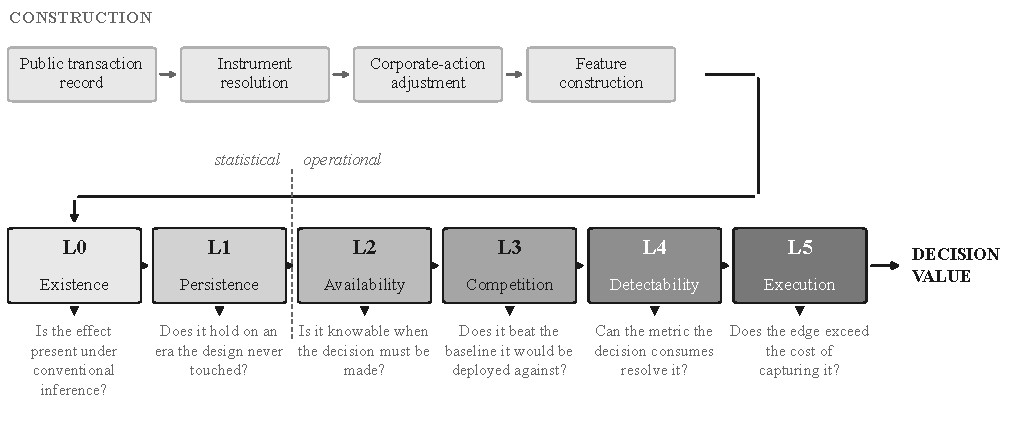
\includegraphics[width=0.95\textwidth]{figures/figure_1_framework.pdf}
\caption{The deployment-validation architecture. The upper row constructs the measurement; the lower row spends it against six ascending constraints, each stated as the question it asks. Constraints $L_0$ and $L_1$ are statistical and interrogate the sample; $L_2$ through $L_5$ are operational and interrogate the decision. An application has decision value through constraint $k$ if it clears constraints 1 to $k$, so the reported quantity is the index of the first constraint it fails. Because the sequence is ordered, attrition is cumulative and the level at which an application stops is a complete statement of what the data was worth in that use.}
\label{fig:framework}
\end{figure*}

\section{Related Work}
\label{sec:related_work}

\subsection{Replication and the Credibility of Empirical Findings}
The credibility of empirical asset pricing has been scrutinized extensively. \cite{hou2020replicating} showed that standard factor models fail to explain anomalous returns when microcap influences are eliminated through NYSE breakpoints and value-weighting. Conversely, \cite{jensen2023there} argued that Bayesian hierarchical modeling of the factor zoo restores replicability for a substantial fraction of documented characteristics. \cite{bowles2024anomaly} analyzed anomaly decay relative to public discovery dates, while \cite{chai2026understanding} explored structural impediments to direct replication in financial econometrics. \cite{chopra2023null} documented the severe publication penalty imposed on null results, explaining why systematic studies of failed deployments remain scarce. These studies focus on whether an anomaly exists across broad cross-sections, but leave unexamined the fate of anomalies that clear statistical tests.

\subsection{Institutional Frictions and Implementation Costs}
A parallel literature evaluates individual implementation frictions across broad collections of candidate signals. \cite{muravyev2025anomalies} examined short-sale borrowing costs across 162 anomalies, showing that an average monthly return of +0.14\% before fees becomes $-0.01$\% net of borrow constraints. \cite{kaplanski2023race} documented the costs of execution delay as market participants compete for liquidity, and \cite{penasse2022understanding} developed theoretical models of alpha decay post-publication. In machine learning asset pricing, \cite{bagnara2024asset} identified transaction costs and look-ahead data leakage as primary drivers of inflated out-of-sample claims. \cite{sak2024exploring} applied portfolio-level shrinkage to prune factor zoos, while \cite{azevedo2023stock} and \cite{li2024replicating} demonstrated substantial geographical attrition across international markets and Chinese A-shares. These contributions test single frictions across many predictors; our work tests an ordered hierarchy of six frictions on a single dataset.

\subsection{Forecast Evaluation, Densities, and Proper Scoring Rules}
Evaluating forecasts in production environments demands rigorous scoring protocols. \cite{waghmare2026proper} surveyed proper scoring rules for density and point forecast evaluation, emphasizing that scoring rules must be strictly consistent with the decision-maker's loss function. \cite{allen2025tail} established tail-calibration tests for probabilistic forecasts, while \cite{arnold2024decompositions} developed exact decompositions of the Continuous Ranked Probability Score (CRPS) to attribute skill improvements across reliability and resolution components. \cite{goncalves2025bootstrapping} analyzed out-of-sample predictability under real-time data revision schedules, and \cite{arian2024backtest} evaluated backtest overfitting and false discovery risks in machine learning strategies.

\subsection{Alternative Data and Institutional Flow in Emerging Markets}
\cite{coyle2024is} reviewed frameworks for establishing the empirical value of data assets, while \cite{sun2024alternative} categorized alternative data applications in enterprise decision systems. In market microstructure, \cite{ghachem2025estimation} advanced the estimation of informed trading models, and \cite{ding2025forecasting} demonstrated the utility of regime-switching volatility architectures across international equity markets.

Focusing specifically on the Indian equity market, \cite{raizada2025trade} demonstrated that foreign institutional investors exhibit positive-feedback trading behaviors consistent with an informational disadvantage relative to domestic participants. \cite{thapa2026policy} investigated institutional flow adjustments surrounding macroeconomic policy announcements, \cite{dey2024study} quantified institutional responses to market risk, and \cite{maheshwari2026fii} documented the structural transition from Foreign Institutional Investor (FII) dominance to Domestic Institutional Investor (DII) absorption. These studies rely primarily on daily market-wide aggregates; our work evaluates proprietary transaction-level settlement records.

\section{Dataset and Empirical Framework}
\label{sec:data}

\subsection{Depository Settlement Records}
The empirical foundation of this study is a complete, proprietary transaction-level record of foreign institutional equity trades in India, spanning January 1, 2011 to March 31, 2025. The dataset encompasses 25,155,785 settled trades across 5,960 individual instrument identifiers. Each record provides the trade execution date, the custodian settlement reporting date, the instrument identifier, a masked participant identifier, trade direction (buy/sell), and traded value in local currency. Unlike public exchange data, which provides only daily aggregate volume by category, this record allows the construction of entity-level composition metrics and participant-specific concentration indices.

\subsection{Masked Participant Persistence and Identity Constraints}
A key property of masked transaction records is the validity of participant tracking over time. While the raw identifiers appear persistent, an empirical audit on a control group of brokers and clearing members (whose population is bounded in the low hundreds) revealed 22,262 distinct masked identifiers over 171 months, with a median entity lifetime of exactly one month. Foreign institutional identifiers exhibited identical behavior across 363,663 distinct masks. Because depository custodians re-mint identifier masks monthly for privacy, all entity concentration and composition statistics utilized in this study are strictly restricted to within-day windows to prevent spurious cross-temporal tracking.

\subsection{Universe Selection and Corporate Actions}
Asset returns are computed from daily exchange closing prices. Corporate actions (splits, bonus issues, dividends, and rights offerings) were verified against observed price adjustment ratios, with an automated guard discarding any post-adjustment daily return exceeding 50\%. Instrument identity is tracked through a point-in-time mapping table with issuer-bounded closure. Fig.~\ref{fig:pipeline} sets out the construction sequence and the gate each stage must clear.

Fig.~\ref{fig:framework} sets out the full architecture: the construction of the measurement, the six ordered constraints, and the question each one asks.

The empirical universe is constructed via an activity-based inclusion rule: an instrument-day enters the modeling universe if it records at least five foreign institutional trades on that day, and an instrument enters an era if it accumulates at least sixty qualifying days within that era. The resulting modeling universe comprises 1,028 unique instruments across 802,806 instrument-days. Because selection operates on trading frequency rather than on past returns, it introduces zero survivorship bias across the structural split.

\begin{figure*}[!t]
\centering
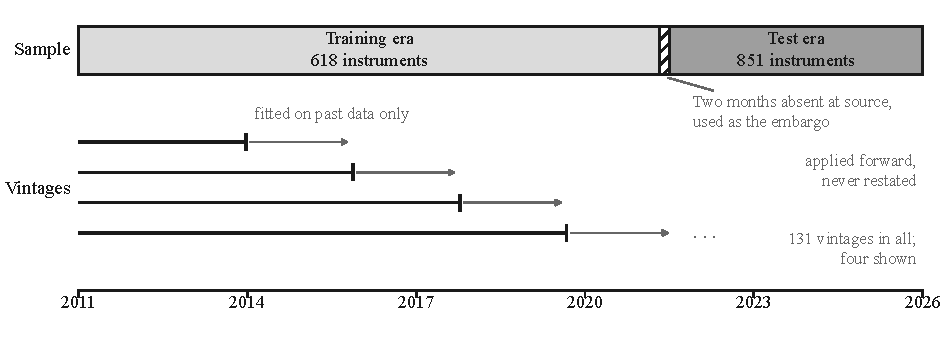
\includegraphics[width=0.88\textwidth]{figures/figure_2_design.pdf}
\caption{Frozen split, embargo, and walk-forward vintage design. Parameters, thresholds, and specifications are estimated exclusively on data through April 30, 2021 (the training era). A two-month operational embargo (May--June 2021) buffers against look-ahead bias across a structural break. The test era commences July 1, 2021, and runs through March 31, 2025. Parameters are frozen into dated vintages and evaluated forward without restatement.}
\label{fig:design}
\end{figure*}

\subsection{Frozen Split and Walk-Forward Vintages}
To eliminate look-ahead bias and data snooping, the dataset is divided into two distinct chronological eras separated by an embargo, as illustrated in Fig.~\ref{fig:design}:
\begin{itemize}
    \item \textbf{Training Era (Jan 1, 2011 -- Apr 30, 2021):} Covers 618 instruments across 508,563 instrument-days. All hyperparameters, model architectures, screening thresholds, and backtest gates were fixed permanently on this sample.
    \item \textbf{Operational Embargo (May 1, 2021 -- Jun 30, 2021):} A two-month structural buffer during which data is omitted at source to separate estimation from out-of-sample testing.
    \item \textbf{Test Era (Jul 1, 2021 -- Mar 31, 2025):} Covers 851 instruments across 294,243 instrument-days. Only 441 instruments appear in both eras, ensuring that out-of-sample validation occurs across a substantially shifting cross-section.
\end{itemize}

Three months within the test era contained an invalid directional trade flag (representing 3.004\% of total trades); these records were dropped entirely rather than imputed. All operational parameters are sealed into dated vintages fitted strictly on past observations and executed forward.

\subsection{Latent Regime Model and Hazard Architecture}
For applications requiring state-space conditioning, latent flow regimes are identified using a three-state Gaussian Hidden Markov Model (HMM) with diagonal covariance. The model is estimated on four daily stock-level features: signed flow persistence, mean trade size relative to the instrument baseline, and participant concentration on the buy side and on the sell side. Estimation is performed via the Expectation-Maximization (EM) algorithm with five random restarts on contiguous blocks of at most 400 days per instrument within the training era. States are labeled deterministically by ordering on fitted flow persistence, yielding buying, selling, and neutral states. The fitted transition matrix demonstrates high persistence, with diagonal probabilities of 0.954, 0.952, and 0.978, implying average dwell times of 22, 21, and 45 trading days, respectively.

In production evaluation, state probabilities are computed via the causal forward recursion without retrospective smoothing. Filtered online states agree with smoothed offline states on 91.3\% of stock-days. A hazard prediction layer forecasts episode termination over a forward $k$-day horizon using a gradient-boosted decision tree ensemble (200 trees, learning rate 0.05) retrained annually on completed episode histories ending at least ten days prior to the evaluation year.

\section{The Six Deployment Constraints}
\label{sec:protocol}

\subsection{Formalization of the Friction Hierarchy}
Each empirical application pairs a statistical significance test with an operational decision-value test on the exact same data sample. Decision value is evaluated ordinally across the six constraints:

\subsubsection{Level 0: Existence (Screening Regression)}
Statistical existence is tested via high-dimensional panel regression. For instrument $i$ on day $t$, let $z_{i,t}$ denote the standardized response variable:
\begin{equation}
z_{i,t} = \alpha_i + \gamma_t + \beta \cdot \text{Share}_{i,t} + \bm{\theta}^\top \mathbf{X}_{i,t} + \varepsilon_{i,t},
\label{eq:panel_reg}
\end{equation}
where $\alpha_i$ and $\gamma_t$ are instrument and date fixed effects, $\text{Share}_{i,t}$ is the foreign institutional fraction of total turnover, and $\mathbf{X}_{i,t}$ controls for log-turnover. Standard errors are clustered on trading date to accommodate arbitrary cross-sectional correlation. The screening threshold is set at $|t| \ge 2.50$, incorporating a Bonferroni adjustment for multiple screening cells.

\subsubsection{Level 1: Out-of-Sample Persistence}
Equation~\eqref{eq:panel_reg} is evaluated across both the training and test eras. A sign flip in the estimated coefficient $\beta$ between eras constitutes an immediate structural failure, regardless of nominal statistical significance.

\subsubsection{Level 2: Availability (Operational Decision Lag)}
Custodial reporting delays mean that transaction records are not instantaneous. The actual knowable lag $L$ is measured empirically from depository timestamps. Equation~\eqref{eq:panel_reg} is re-estimated substituting $\text{Share}_{i,t-L}$ in place of the contemporaneous term, holding all fixed effects, controls, and clustering structures constant.

\subsubsection{Level 3: Baseline Competition}
At the market level, the aggregate flow variable $F_t$ is constructed from settled trades:
\begin{equation}
F_t = \frac{\sum_{k} (\text{Buy}_{k,t} - \text{Sell}_{k,t})}{\frac{1}{250}\sum_{s=1}^{250} |\text{Gross}_{t-s}|},
\label{eq:market_flow}
\end{equation}
where the numerator is net institutional flow and the denominator is the trailing 250-day average gross volume. The predictive risk specification regresses absolute index returns $|r_{t+1}|$ on the lagged flow signal:
\begin{equation}
|r_{t+1}| = \alpha + \beta_1 F_{t-L} + \beta_2 F_{t-L}^- + \sum_{j=0}^{4} \phi_j |r_{t-j}| + \psi \text{VIX}_t + \varepsilon_{t+1},
\label{eq:risk_reg}
\end{equation}
where $F^- = \min(F, 0)$ captures asymmetric downside flow impacts, and standard errors are Newey--West with 10 lags.

In Level 3, the resulting forecast is competed directly against an established operational baseline (e.g., GJR-GARCH or an asymmetric volatility model) using the Diebold--Mariano test on CRPS differentials with a gate threshold of $t_{\text{DM}} \le -2.0$.

\subsubsection{Level 4: Detectability (Consuming Metric and Ablation)}
An effect must be resolvable within the operational metric consumed by risk managers or portfolio optimizers. Where a structural mechanism is proposed, detectability is evaluated via strict ablation: re-running the complete modeling pipeline with the specific feature or mechanism removed, measuring the net score differential $\Delta \mathcal{S}$.

\subsubsection{Level 5: Execution (Break-Even Cost Analysis)}
We state the form of the cost model rather than implying a calibrated cost stack. Net profit is gross profit less a flat one-way charge applied linearly to gross turnover, $\text{Net}_t = \text{Gross}_t - c \cdot \text{Turnover}_t$, with position weights capped at 5\% and trades executed close-to-close at $L=1$. The charge is symmetric across buys and sells; it is not decomposed into brokerage, exchange fees, securities transaction tax, or market impact, it does not scale with order size, and it carries no separate borrow cost on the short leg. On that basis we evaluate the break-even one-way transaction cost $c^*$ at which net trading profit is identically zero:
\begin{equation}
c^* = \frac{\mathbb{E}[\text{Gross Profit}]}{\mathbb{E}[\text{Turnover}]},
\label{eq:breakeven}
\end{equation}
expressed in basis points (bp) per unit of turnover. The break-even cost $c^*$ is an invariant property of the strategy itself, which is compared against a conservative institutional execution benchmark for this market ($\sim 15$~bp one-way). We report $c^*$ rather than a net Sharpe ratio because $c^*$ is a property of the strategy while a net figure is a property of the cost assumption: a reader whose execution costs differ can use the first and cannot use the second.

\begin{figure*}[t]
\centering
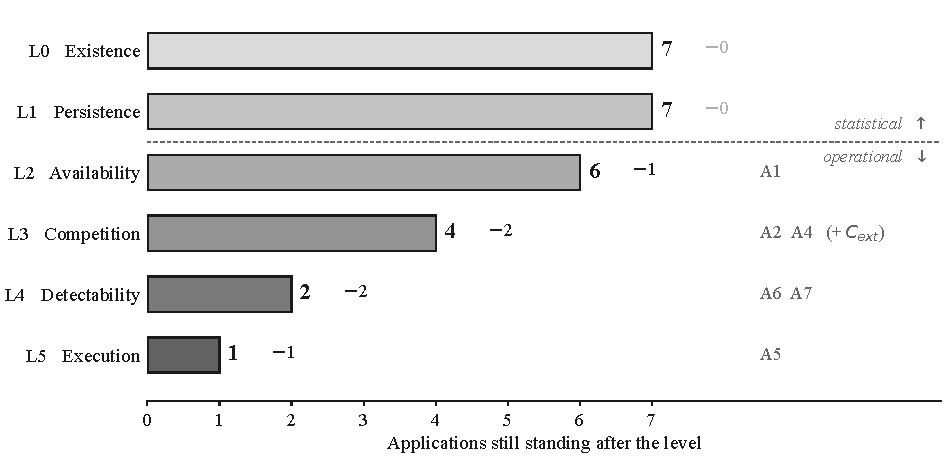
\includegraphics[width=0.88\textwidth]{figures/figure_2_attrition.pdf}
\caption{Attrition ladder across six ascending deployment constraints. Each of the seven applications of the institutional flow dataset ($A_1$, $A_2$, and $A_4$ through $A_8$) is charged to the lowest constraint level it fails to survive; the bar length is the number still standing once that level has been applied. The external non-flow control predictor ($C_{\text{ext}}$, indexed $A_3$ in the artifact registry) is annotated where it fails but is excluded from every count, since it is not an application of the record. All seven survive statistical existence ($L_0$) and out-of-sample persistence ($L_1$), but six fail under the operational deployment constraints ($L_2$--$L_5$). Exactly one application ($A_8$, the aggregate market-level density forecast) survives all six levels.}
\label{fig:attrition}
\end{figure*}

\subsection{Backtest Gating Protocol}
Simulated portfolio execution follows strict timing equations: signals generated at the market close of day $t$ are executed at the close of $t+1$ and receive the close-to-close return of $t+2$ ($L=1$).

All execution engines must pass three automated sanity gates before admission:
\begin{enumerate}
    \item \textbf{Exactness Gate:} The vectorized production engine must generate numerically identical trajectory vectors to an unoptimized per-day loop.
    \item \textbf{Alignment Gate:} An artificial look-ahead oracle signal ($s_t = r_{t+1}$) must generate an extreme Sharpe ratio at lag 0 and collapse to zero at lag 1.
    \item \textbf{Cost Accounting Gate:} A synthetic portfolio with deterministic turnover must satisfy $\text{Net} \equiv \text{Gross} - c \cdot \text{Turnover}$ to machine precision.
\end{enumerate}

\section{Empirical Results and Failure Analysis}
\label{sec:results}

\subsection{Overall Attrition Across the Friction Ladder}
Fig.~\ref{fig:attrition} depicts the progressive attrition of the seven institutional flow applications and the external control predictor across the six deployment levels.

Crucially, \textbf{no application was eliminated at Level 0 (Existence) or Level 1 (Persistence)}. Across all seven applications, statistical significance was confirmed on the training sample and held on the frozen test era. However, attrition began immediately upon entering the operational deployment constraints ($L_2$--$L_5$), with failures distributed across four distinct levels.

\subsection{Level 2: Availability Failure ($A_1$)}
Application $A_1$ utilizes the institutional turnover share to predict next-day idiosyncratic stock volatility across 577,245 instrument-days. In the contemporaneous specification (where trades on day $t$ are assumed known at the close of day $t$), the predictor produces a massive, highly stable negative coefficient: $t = -5.53$ in the full sample, $t = -4.42$ in training, and $t = -3.25$ in testing.

However, depository timestamp audits reveal that on a value-weighted basis, only 0.13\% of daily trades are reported by the market close of day $t$. 94.30\% are reported by the close of $t+1$, and 97.51\% by $t+2$. Thus, $t+2$ represents the earliest feasible operational deployment lag.

\begin{table}[!t]
\caption{\textbf{Impact of Operational Availability Lag on Predictive Significance (Application $A_1$)}}
\label{tab:table1}
\setlength{\tabcolsep}{4pt}
\begin{tabularx}{\columnwidth}{@{}Xrrr@{}}
\hline
\textbf{Information set} & \textbf{Full sample} & \textbf{Training} & \textbf{Test era} \\
\hline
Contemporaneous (lag 0) & $-5.53$ & $-4.42$ & $-3.25$ \\
Operational lag ($t-2$) & $-0.43$ & $-0.09$ & $-0.44$ \\
\hline
\multicolumn{4}{@{}p{\columnwidth}@{}}{\footnotesize\textit{Entries are $t$-statistics on the foreign institutional share coefficient in \eqref{eq:panel_reg}, controlling for instrument and date fixed effects and log-turnover, with standard errors clustered on trading date. Both rows use the same panel, the same fixed effects, the same controls and the same clustering; they differ only in the lag at which the predictor is taken. The contemporaneous effect does not weaken at the physically knowable two-day lag---it disappears.}}
\end{tabularx}
\end{table}

Fig.~\ref{fig:availability} traces the coefficient and its $t$-statistic across every lag from $t{-}0$ to $t{-}5$, so the collapse can be read as a profile rather than as two endpoints. As shown in Table~\ref{tab:table1}, re-estimating the exact panel regression at the operational lag of $t-2$ causes the statistical relationship to collapse to zero ($t = -0.43$ full sample, $-0.09$ training, $-0.44$ test). The collapse is not an artifact of the variance estimator. On the full sample, two-way clustering on instrument and date gives $t = -5.20$ contemporaneously against $-0.42$ lagged, and a stationary date-block bootstrap gives $t = -6.47$ against $-0.47$; White standard errors give $-6.29$ against $-0.45$. Under every estimator the contemporaneous effect is strong and the deployable one is absent, which locates the signal as contemporaneous market microstructure rather than a tradable forecast.


\begin{figure}[!t]
\centering
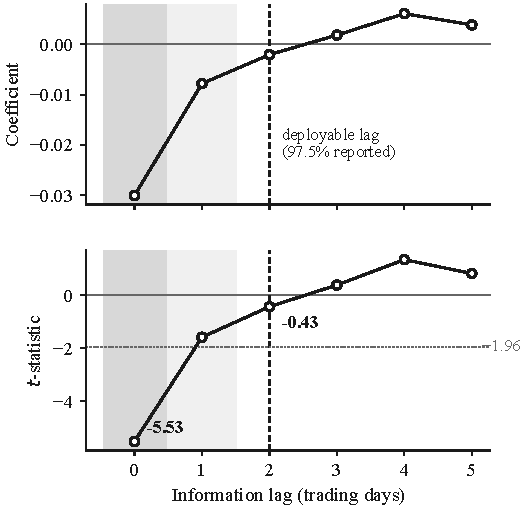
\includegraphics[width=\columnwidth]{figures/figure_3_availability.pdf}
\caption{Application $A_1$ across information lags. The specification of \eqref{eq:panel_reg} is re-estimated at each lag with the panel, fixed effects, controls, and clustering held identical; only the information set changes. Shading marks the share of a day's flow value actually reported by that lag: 0.13\% by $t{+}0$ and 94.30\% by $t{+}1$. The dashed line marks the earliest deployable lag, $t{-}2$, at which 97.51\% has been reported. The coefficient does not merely attenuate---it crosses zero by lag three.}
\label{fig:availability}
\end{figure}

\subsection{Level 3: Baseline Competition Failures ($A_2$, $A_4$, and $C_{\text{ext}}$)}

\subsubsection{Controlled Density Forecast Pair ($A_8$ vs. $A_2$)}
Applications $A_8$ and $A_2$ share the identical underlying statistical screen: the market-level net flow variable \eqref{eq:market_flow} regressed on index absolute returns via \eqref{eq:risk_reg}. The screening regression yields $t = -4.83$ in the full sample, $t = -2.53$ in training, and $t = -2.51$ in testing, easily clearing the $|t| \ge 2.50$ Bonferroni screening hurdle.

Both applications apply the identical flow tilt over the exact same 2,235 scored trading days, differing solely in the sophistication of the baseline volatility model:
\begin{itemize}
    \item $A_8$ competes against an Exponentially Weighted Moving Average (EWMA) baseline.
    \item $A_2$ competes against an Asymmetric GJR-GARCH baseline.
\end{itemize}

\begin{table}[!t]
\caption{\textbf{The Same Flow Predictor Evaluated Against Two Competing Baselines}}
\label{tab:table2}
\setlength{\tabcolsep}{3pt}
\begin{tabularx}{\columnwidth}{@{}Xrr@{}}
\hline
\textbf{Evaluation metric} & \textbf{EWMA base ($A_8$)} & \textbf{GJR-GARCH ($A_2$)} \\
\hline
Diebold--Mariano $t$ & $-2.22$ (\textbf{pass}) & $+0.28$ (\textbf{fail}) \\
Training score advantage ($\times 100$) & $-0.0024$ & $-0.0001$ \\
Test-era score advantage ($\times 100$) & $-0.0004$ & $+0.0002$ (\textbf{fail}) \\
Kupiec coverage $p$ (5\%, 1\%) & 0.375, 0.248 & 0.486, 0.248 \\
Scored trading days & 2,235 & 2,235 \\
\hline
\multicolumn{3}{@{}p{\columnwidth}@{}}{\footnotesize\textit{The Diebold--Mariano gate is $t \le -2.0$; a negative score advantage favors the tilted model. Both columns carry the identical two-term flow tilt, the identical comparison model and the identical 2,235 scored days; only the baseline density differs. Against the simpler EWMA baseline the tilt clears every leg of its pre-registered gate. Against the better-specified GJR-GARCH baseline the incremental value disappears and the test-era sign reverses---a failure under the pre-registration regardless of magnitude.}}
\end{tabularx}
\end{table}

Table~\ref{tab:table2} shows that against the EWMA baseline the flow signal clears all three legs of its pre-registered gate ($t_{\text{DM}} = -2.22$ on the 2,235-day common window; $-2.35$ on the 2,739 days the engine scores in its own right). However, against the GJR-GARCH baseline, the Diebold--Mariano statistic flips positive ($+0.28$), and the test-era score differential degrades (+0.0002). Because GJR-GARCH already absorbs asymmetric volatility persistence, the flow signal provides zero incremental value. Fig.~\ref{fig:competition} plots the cumulative score advantage of both comparisons, which separates the two verdicts visually and also exposes the time profile of the surviving advantage. \textit{Incremental forecasting value is a property of the model pair, rather than an intrinsic attribute of the data.}


\begin{figure}[!t]
\centering
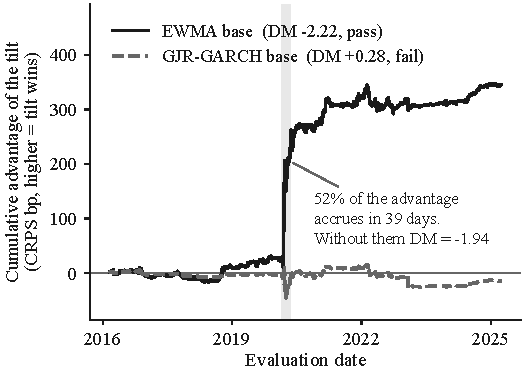
\includegraphics[width=\columnwidth]{figures/figure_4_competition.pdf}
\caption{Cumulative score advantage of the identical flow tilt against two baselines over the identical 2,235 scored days; a rising path means the tilt is outscoring its baseline. Only the baseline density differs between the two lines. The path additionally shows \emph{when} the advantage accrues, which a single summary statistic cannot: shading marks March--April 2020.}
\label{fig:competition}
\end{figure}

\subsubsection{Discrete-Time Hazard Model vs. Trivial Rule ($A_4$)}
Application $A_4$ employs a walk-forward gradient-boosted hazard model to forecast flow episode termination. As reported in Table~\ref{tab:table3}, the machine learning model demonstrates genuine out-of-sample statistical discrimination, achieving an Area Under the ROC Curve (AUC) of 0.657 in the test era (compared to 0.569 for an age-only baseline) and a paired log-loss statistic of 14.42.

\begin{table}[!t]
\caption{\textbf{Forecast Discrimination vs. Decision Value in Episode Hazard Modeling (Application $A_4$)}}
\label{tab:table3}
\setlength{\tabcolsep}{3pt}
\begin{tabularx}{\columnwidth}{@{}Xrr@{}}
\hline
\textbf{Metric} & \textbf{GBDT model} & \textbf{Age heuristic} \\
\hline
AUC (pooled sample) & 0.647 & 0.569 \\
AUC (training era) & 0.637 & --- \\
AUC (test era) & 0.657 & --- \\
Paired log-loss statistic & $+14.42$ & --- \\
Test anticipation gain (bp/episode) & $-18$ & $+16$ \\
Paired difference, 402 episodes (bp) & $-31$ ($t=-1.85$) & --- \\
\hline
\multicolumn{3}{@{}p{\columnwidth}@{}}{\footnotesize\textit{The learned model discriminates better out of sample than in (AUC 0.657 vs.\ 0.637), which rules out memorization, and beats the duration-only baseline decisively (0.647 vs.\ 0.569). The operational policy derived from it nonetheless underperforms a three-line age-based rule by 31~bp on the episodes both act upon. Comparing each rule against zero separately would have reported the model as the better of two positives; only the paired comparison on shared events recovers the ordering.}}
\end{tabularx}
\end{table}

Fig.~\ref{fig:discrimination} places the two evaluations side by side. Despite this statistical skill, when converted into an operational execution rule, the model delivers an anticipation return of $-18$~bp per episode, losing by 31~bp to a trivial three-line heuristic rule ($+16$~bp) on the 402 common episodes both act upon. A conventional evaluation comparing the model against zero would have erroneously declared success.

\subsubsection{External Control Predictor ($C_{\text{ext}}$)}
The external control predictor uses 5-day lagged foreign market returns (S\&P 500) to predict domestic equity volatility. The initial screening regression yields extraordinarily stable coefficients across eras ($t = -3.86$ full, $-2.91$ training, $-4.46$ test). However, when evaluated in a full density forecast engine, it achieves a score differential of $+1.58$ against the $-2.0$ gate threshold. The non-flow control predictor fails at the exact same competition constraint as the internal flow models, demonstrating that deployment attrition is systemic rather than dataset-specific.


\begin{figure*}[!t]
\centering
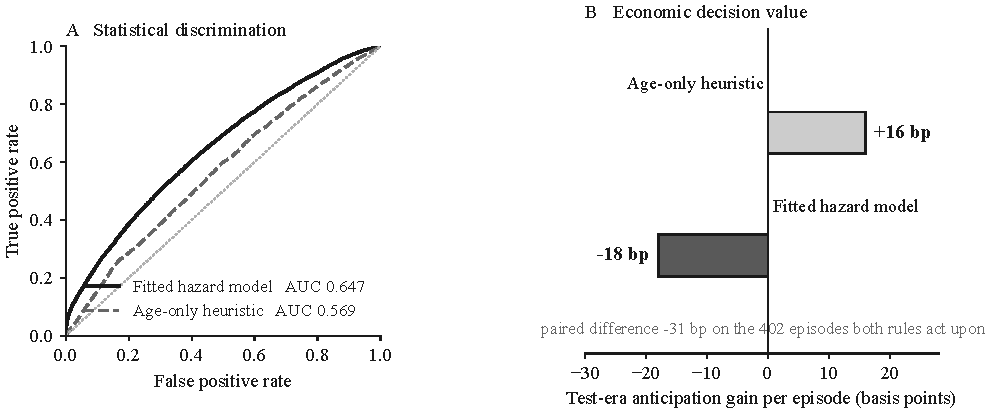
\includegraphics[width=0.92\textwidth]{figures/figure_5_discrimination_vs_decision.pdf}
\caption{Application $A_4$: statistical discrimination against economic decision value. (a) Receiver operating characteristic curves computed from the model's own out-of-sample predictions; the fitted hazard model dominates the age-only heuristic. (b) The anticipation gain each rule actually earns in the test era. The ordering reverses. Comparing each rule against zero separately would have reported the model as the better of two positives; only the paired comparison on the 402 episodes both rules act upon recovers the ordering.}
\label{fig:discrimination}
\end{figure*}

\subsection{Level 4: Detectability Failures ($A_6$ and $A_7$)}
Applications $A_6$ and $A_7$ survive baseline competition but fail because downstream decision metrics cannot resolve their signal.

In $A_6$, a participant-composition feature block produces a substantial top-minus-bottom quintile spread of 74.8~bp ($t = 2.86$) on non-overlapping episodes. However, its incremental Information Coefficient (IC) across the full panel is only 0.0012 ($t = 0.67$) against an institutional acceptance threshold of $\text{IC} \ge 0.005$ ($t \ge 2.0$). The effect concentrates exclusively in extreme tails and is unresolvable in bulk scoring.

\begin{table}[!t]
\caption{\textbf{Ablation of State Conditioning in the Stock-Day Density Engine (Application $A_7$)}}
\label{tab:table4}
\setlength{\tabcolsep}{3pt}
\begin{tabularx}{\columnwidth}{@{}Xrrr@{}}
\hline
\textbf{Evaluation stratum} & \textbf{DM stat.} & \textbf{Prob.} & \textbf{Score effect} \\
\hline
Pre-registered primary (uncertain state) & $-0.82$ & 0.4100 & $-0.00004$ \\
Full cross-sectional panel & $+2.90$ & 0.0037 & $+0.00005$ \\
\hline
\multicolumn{4}{@{}p{\columnwidth}@{}}{\footnotesize\textit{The identical density machinery is re-run with the conditioning removed and everything else held fixed. In the pre-registered primary stratum, where the flow-regime mechanism should bind hardest, the conditioned density is statistically indistinguishable from its own ablation ($p = 0.41$). On the full panel it is statistically favored, but by five parts in 100{,}000 of a score whose level is near 0.55.}}
\end{tabularx}
\end{table}

In $A_7$, stock-day flow regimes cluster strongly ($p = 0.005$ against a randomized null). To determine whether this latent mechanism adds value to a downstream predictive density engine, we conduct an exact ablation test. As shown in Table~\ref{tab:table4}, in the pre-registered primary stratum where state uncertainty is greatest, the conditioned model is indistinguishable from its ablation ($t = -0.82$, $p = 0.41$). On the full panel, the statistical advantage is $+0.00005$ on a base score of 0.55---an improvement of one part in eleven thousand. The complex conditioning architecture contributes negligible operational resolution.

\subsection{Level 5: Execution Cost Failure ($A_5$)}
Application $A_5$ implements a mechanical long-short strategy based on within-day institutional concentration. The strategy requires no parametric fitting and generates gross Sharpe ratios of 1.36 in the training era and 1.51 in the test era.

Applying \eqref{eq:breakeven}, the strategy's break-even one-way transaction cost $c^*$ is calculated at 7.33~bp in training and 7.41~bp in testing. Against a one-way benchmark of 15~bp, net performance collapses to Sharpe ratios of $-1.42$ and $-1.53$. Because the signal requires daily rebalancing across hundreds of names, transaction costs exceed the gross alpha by a factor of two. Fig.~\ref{fig:execution} plots the full cost frontier against the itemized stack the strategy would actually pay. For cash-delivery equity the Securities Transaction Tax alone is 10~bp per side; the break-even is therefore unreachable in that instrument, and the execution constraint binds more sharply than a single 15~bp comparison implies.


\begin{figure}[!t]
\centering
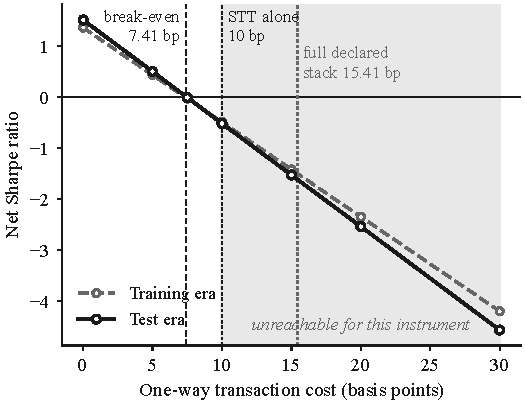
\includegraphics[width=\columnwidth]{figures/figure_6_execution_frontier.pdf}
\caption{Application $A_5$ against the cost frontier it must actually pay. Net Sharpe is linear in the one-way cost because turnover is a property of the book that cost does not change. For cash-delivery equity the Securities Transaction Tax alone is 10~bp per side, which already exceeds the 7.41~bp break-even, so the shaded region is unreachable in the instrument this strategy would have to trade.}
\label{fig:execution}
\end{figure}

\subsection{Characterization of the Surviving Predictor ($A_8$)}
\label{sec:survivor}
Exactly one application survives all six levels: the market-level density forecast ($A_8$) incorporating aggregate net flow \eqref{eq:market_flow} at a two-day reporting lag against an EWMA baseline.

This survival is subject to six boundary conditions, each of which the paper states rather than absorbs:
\begin{enumerate}
    \item \textit{Baseline Sensitivity:} It survives against an EWMA baseline ($t = -2.22$), but fails if scored against a bare baseline without implied volatility ($t = -1.29$).
    \item \textit{Search Multiplicity:} The one-sided $p$-value of 0.0095 adjusts to $p = 0.038$ under Bonferroni/Holm corrections across the four gating engines, and widens to $p = 0.052$ on the common window.
    \item \textit{Sequential Search Costs:} Because gating thresholds were formulated sequentially across research iterations, formal corrections understate the true historical model search space.
    \item \textit{Metric Centrality:} Performance holds under CRPS integrated across the 1st--99th percentiles, representing a central-distribution forecast improvement rather than an extreme-tail risk warning.
    \item \textit{Crisis Concentration:} The advantage is not earned evenly. The 39 trading days of March--April 2020---1.7\% of the scored sample---carry 52\% of the entire cumulative score advantage (Fig.~\ref{fig:competition}). Excluding that window, the score differential moves from $-2.22$ to $-1.94$ and the gate is not cleared. The surviving result is therefore conditional on a single volatility regime as well as on the four accountings below.
    \item \textit{Nested-Model Inference:} The gate compares strictly nested specifications---the tilted model adds two parameters to its own baseline---so the Diebold--Mariano statistic is not distribution-free here. A stationary block bootstrap of the score differential agrees with the gate ($p = 0.028$ on the engine's own window, $p = 0.033$ on the common window), but a Clark--West adjustment for the estimation noise the larger model incurs does not ($t = +1.27$, one-sided $p = 0.10$). Because estimation is expanding-window, the finite-window argument that would license the unadjusted comparison does not apply. We therefore report the survivor as a demonstrated possibility under its pre-registered gate rather than as a confirmed general effect. Fig.~\ref{fig:fragility} collects these accountings on one axis, and Fig.~\ref{fig:rolling} shows the corresponding time profile.
\end{enumerate}

One point runs the other way. Of the four gating engines, $A_8$ alone was left unchanged by two later estimation corrections---an out-of-sample maturity floor and an optimizer path-independence fix---that widened its three siblings from narrow misses into clear failures. A result that does not move when its neighbors move under a correction is a result that was not resting on the defect.

\section{Managerial and Engineering Implications}
\label{sec:implications}
The findings yield four concrete principles for quantitative engineering, risk management, and data procurement.

\textbf{1. Establish the Deployment Lag Before Estimating Significance.} Predictive regressions are routinely estimated contemporaneously or at an assumed one-day lag. Application $A_1$ shows that custodian settlement schedules can impose a mandatory two-day lag, and that the effect does not survive it. Running the first regression at the true deployable lag eliminates non-viable signals before any engineering is committed.

\textbf{2. Benchmark Against Production Systems, Not Null Models.} Vendors typically demonstrate predictive content against weak or naive baselines. Table~\ref{tab:table2} shows the same signal clearing a strict gate against an EWMA model and contributing nothing over a GJR-GARCH system. Data buyers should require evaluation against their own production baseline.

\textbf{3. Aggregate to the Scale of Signal Stability.} The sole surviving application in this study was aggregated to the market level, whereas all stock-level implementations failed at availability, detectability, or execution. When participant entity identifiers are subject to periodic obfuscation or high noise, cross-sectional aggregation acts as an effective noise filter.

\textbf{4. Enforce Mechanism Ablation in Risk Validation.} When a risk model is sold on a specific structural innovation---HMM regime conditioning, say---validation should mandate an exact ablation. Table~\ref{tab:table4} shows such a mechanism consuming substantial computation while contributing under 0.01\% of predictive score.

\section{Limitations and Future Research}
\label{sec:limitations}
Several methodological limitations contextualize this work:
\begin{itemize}
    \item \textit{Single Dataset and Market:} While the logical ordering of the friction ladder is universally applicable, the specific failure proportions represent an empirical case study of one dataset in the Indian market.
    \item \textit{Staggered Difference-in-Differences:} The flow episode framework features heterogeneous start and end dates. Modern staggered treatment effect estimators \cite{aguilarloyo2025comparative, dechaisemartin2026differenceindifferences} were not applied.
    \item \textit{Search Space Pricing:} While individual engine gates were pre-registered, the broader historical exploration of strategy books was not penalized via formal Deflated Sharpe Ratio or White's Reality Check metrics \cite{arian2024backtest, anghel2021data, hollstein2022world}.
    \item \textit{Tail Calibration Scoring:} Density evaluation relied primarily on CRPS; integrating tail-weighted scoring rules \cite{allen2025tail, arnold2024decompositions} represents a natural technical extension.
    \item \textit{Execution Instrument Unmodeled:} The backtest applies a generic one-way charge on turnover and does not specify a traded instrument. Whether $A_5$ would be implemented in cash-delivery equity, in single-stock or index futures, or intraday materially changes the applicable cost stack---securities transaction tax, stamp duty, and short-leg borrow differ sharply across those routes in this market. The 15~bp figure is a conservative round-number benchmark rather than a calibrated estimate for any one of them. The break-even $c^*$ of 7.33--7.41~bp is reported precisely so that the verdict can be re-derived under a reader's own cost stack; at any one-way cost above roughly 7.4~bp the conclusion is unchanged.
    \item \textit{Nested-Model Test Selection:} The surviving application's gate was pre-registered as a Diebold--Mariano comparison, which the nesting of the two specifications does not strictly license. The Clark--West disagreement reported in Section~\ref{sec:results} is left standing rather than resolved by substituting a test after the fact; settling it requires re-estimating the engine family on a rolling rather than expanding window.
\end{itemize}

\section{Conclusion}
\label{sec:conclusion}
This study tracked a 14-year, 25.15-million-trade record of foreign institutional equity flows across an ordered hierarchy of six deployment constraints. While every application passed conventional statistical significance and out-of-sample persistence without attrition, six of seven applications failed when subjected to operational frictions: one at data availability, two at baseline competition, two at metric detectability, and one at transaction cost execution. Exactly one application survived, subject to strict baseline and aggregation boundaries.

By grounding every reported empirical metric in a primary, verifiable computational artifact, this work demonstrates that the loss of predictive value is a systematic property of the deployment pipeline rather than a flaw in the underlying statistical data. Quantitative practitioners must evaluate alternative data directly through the lens of institutional constraints.

%% =====================================================================
%% TODO BEFORE SUBMISSION (1 of 2) -- DATA/CODE AVAILABILITY STATEMENT.
%% IEEE Access's reproducibility initiative awards Code Available / Code
%% Reviewed badges for artifacts deposited with a persistent DOI. Nothing
%% below is rendered until the block is uncommented and the URL filled in.
%%
%% \section*{Data and Code Availability}
%% The raw depository settlement record cannot be redistributed <STATE WHY>.
%% The derived artifacts, cryptographic digests, and extractor code that bind
%% every reported number to its producing computation are available at
%% <URL / DOI>. <NAME WHICH DERIVED ARTIFACTS ARE INCLUDED.>
%% =====================================================================
%%
%% TODO BEFORE SUBMISSION (2 of 2) -- DATA ACCESS BASIS.
%% The acknowledgment below names "data depository administrators" without
%% stating the access basis. An editor's COI/ethics screen will ask how an
%% unaffiliated, unfunded author obtained proprietary FII settlement data.
%% Replace the paragraph with a one-line statement of the actual basis
%% (institutional project / licence / employer), and check it against the
%% \tfootnote no-funding declaration and the "Independent Researcher"
%% affiliation for consistency.
%% =====================================================================
\appendices
\section{Supplementary Figures}
\label{app:supplementary}
The four figures collected here support claims made in the main text. Each is
regenerated from the accompanying artifact by
\texttt{reproduction/reproduce\_figures.py}, which reads only the derived
panels distributed with it.

\subsection{Time Profile of the Surviving Advantage}
Section~\ref{sec:survivor} reports that the surviving application's score
advantage is concentrated in a single volatility regime. Fig.~\ref{fig:rolling}
gives the time-series form of that statement. A rolling 252-day mean of the
score differential is near zero for the first four years of the evaluation
window, rises sharply through the March 2020 regime, and decays across the test
era, with a negative excursion during 2023. The concentration is therefore not
an artifact of the cumulative representation in Fig.~\ref{fig:competition}: the
advantage genuinely accrues in bursts, and a single summary statistic computed
over the full window averages across regimes in which the predictor behaves
very differently.

\begin{figure}[!t]
\centering
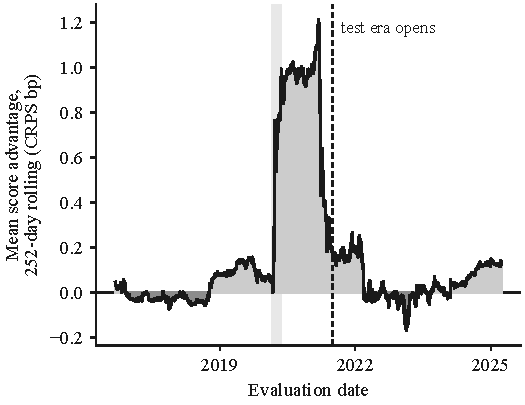
\includegraphics[width=\columnwidth]{figures/figure_7_survivor_rolling.pdf}
\caption{Rolling 252-day mean score advantage of the surviving application $A_8$ against its baseline. Positive values indicate that the flow tilt is outscoring the baseline. The advantage is episodic rather than steady, which is the time-series form of the crisis-concentration condition reported in Section~\ref{sec:survivor}.}
\label{fig:rolling}
\end{figure}

\subsection{Inferential Status Under Stricter Accounting}
The five inferential conditions enumerated in Section~\ref{sec:survivor} are
easier to weigh when placed on a common axis. Fig.~\ref{fig:fragility} plots
each accounting against the conventional five per cent threshold. Two of the
five do not clear it: the common-window multiplicity adjustment at $p = 0.052$,
and the Clark--West correction for nested-model comparison at $p = 0.10$. We
include the figure because the alternative---reporting only the accountings
that pass---would misrepresent how much weight the surviving result can bear.
A reader who regards either of the two failing accountings as decisive should
read the study as reporting no surviving application rather than one.

\begin{figure}[!t]
\centering
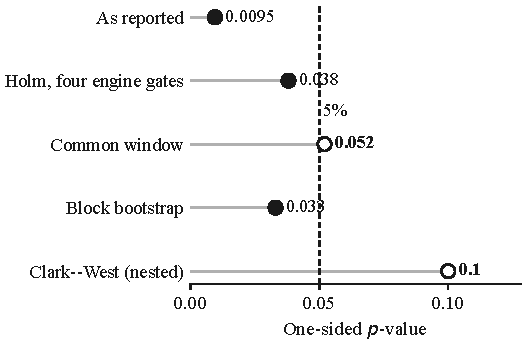
\includegraphics[width=\columnwidth]{figures/figure_8_survivor_fragility.pdf}
\caption{The surviving application's inferential status under successively stricter accounting. Filled markers clear the conventional five per cent threshold; hollow markers do not. Two of five accountings do not clear it.}
\label{fig:fragility}
\end{figure}

\subsection{Construction and Its Validation Gates}
Fig.~\ref{fig:pipeline} sets out the construction sequence described in
Section~III and marks the stages that are verified rather than trusted. Two
are worth isolating. Instrument identity is resolved through a point-in-time
map with issuer-bounded closure, which yields 1,784 validity intervals with no
overlapping assignments; without the issuer bound, closure over a recycled
ticker would chain two unrelated issuers into one synthetic instrument with a
spurious fourteen-year history. Corporate-action factors are checked against
the observed pre/post price ratio rather than applied on the strength of the
filing alone: 805 are confirmed, 291 are unverifiable because no clean ratio is
observable around the ex-date, and seven contradict the filing. The seven are
flagged and reported rather than silently corrected, on the principle that a
diagnostic is read-only and a data repair is never bundled with the analysis
that motivated it.

\begin{figure}[!t]
\centering
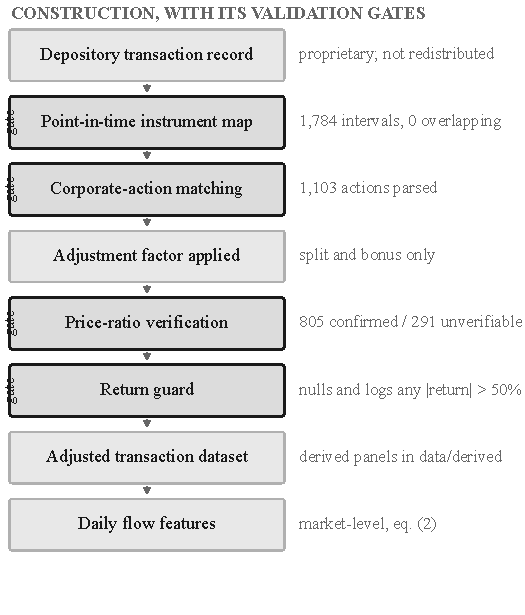
\includegraphics[width=\columnwidth]{figures/figure_9_data_pipeline.pdf}
\caption{Data construction and its validation gates. Bordered stages are verified rather than trusted. Of 1,103 parsed corporate actions, 805 are confirmed against the observed price ratio, 291 are unverifiable, and 7 contradict the filing.}
\label{fig:pipeline}
\end{figure}

\subsection{The External Control Predictor}
The control predictor is a five-day foreign index return used to forecast
next-week domestic realised volatility. It is not an application of the flow
record, and it was run through identical machinery precisely so that the flow
record's failures could be distinguished from failures of the evaluation
apparatus. Fig.~\ref{fig:control} shows both halves of the result. Its
screening regression is among the most era-stable coefficients the programme
produced and is stronger out of sample than in; the density engine built on it
nonetheless fails at the competition constraint, with the falling cumulative
path indicating that the tilted engine scores worse than its own baseline. A
predictor drawn from outside the record entirely therefore fails at the same
constraint and by the same mechanism as two of the flow applications, which is
the basis for treating deployment attrition as a property of the evaluation
transition rather than of this dataset.

\begin{figure}[!t]
\centering
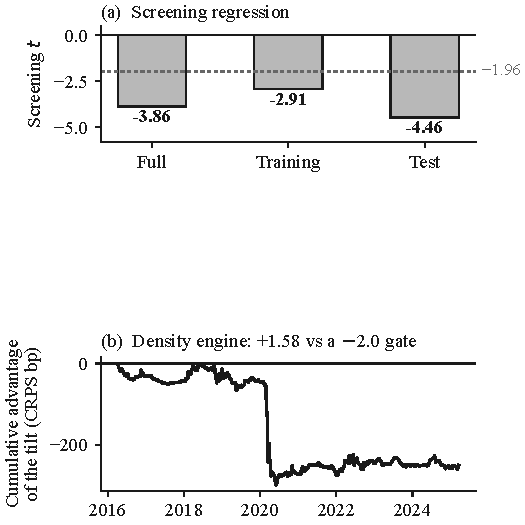
\includegraphics[width=\columnwidth]{figures/figure_10_external_control.pdf}
\caption{The external non-flow control predictor $C_{\text{ext}}$. (a) The screening regression is strong and stable across eras. (b) The density engine built on it nonetheless fails at the competition constraint, the falling path indicating that the tilted engine scores worse than its own baseline.}
\label{fig:control}
\end{figure}

\section*{Acknowledgment}
The authors thank the data depository administrators and the quantitative research colleagues who provided foundational infrastructure support during this investigation.

\begin{thebibliography}{29}
\providecommand{\url}[1]{#1}
\expandafter\ifx\csname urlstyle\endcsname\relax\else\urlstyle{same}\fi

\bibitem{hou2020replicating} K. Hou, C. Xue, and L. Zhang, ``Replicating Anomalies,'' Rev. Financ. Stud., vol. 33, no. 5, pp. 2019--2133, May 2020, doi: \url{10.1093/rfs/hhy131}.

\bibitem{jensen2023there} T. I. Jensen, B. Kelly, and L. H. Pedersen, ``Is There a Replication Crisis in Finance?,'' J. Finance, vol. 78, no. 5, pp. 2465--2518, Oct. 2023, doi: \url{10.1111/jofi.13249}.

\bibitem{bowles2024anomaly} B. Bowles, A. V. Reed, M. C. Ringgenberg, and J. R. Thornock, ``Anomaly Time,'' J. Finance, vol. 79, no. 5, pp. 3543--3579, Oct. 2024, doi: \url{10.1111/jofi.13372}.

\bibitem{chai2026understanding} D. Chai, S. Ali, M. Brosnan, and T. Hasso, ``Understanding researchers' perceptions and experiences in finance research replication studies: A pre-registered study,'' Pac.-Basin Finance J., vol. 96, p. 103061, Feb. 2026, doi: \url{10.1016/j.pacfin.2026.103061}.

\bibitem{chopra2023null} F. Chopra, I. Haaland, C. Roth, and A. Stegmann, ``The Null Result Penalty,'' Econ. J., vol. 134, no. 657, pp. 193--219, Dec. 2023, doi: \url{10.1093/ej/uead060}.

\bibitem{muravyev2025anomalies} D. Muravyev, N. D. Pearson, and J. M. Pollet, ``Anomalies and Their Short-Sale Costs,'' J. Finance, vol. 80, no. 6, pp. 3639--3694, Dec. 2025, doi: \url{10.1111/jofi.13501}.

\bibitem{kaplanski2023race} G. Kaplanski, ``The race to exploit anomalies and the cost of slow trading,'' J. Financ. Mark., vol. 62, p. 100754, Jan. 2023, doi: \url{10.1016/j.finmar.2022.100754}.

\bibitem{penasse2022understanding} J. P{\'e}nasse, ``Understanding Alpha Decay,'' Manag. Sci., vol. 68, no. 5, pp. 3966--3973, May 2022, doi: \url{10.1287/mnsc.2022.4353}.

\bibitem{bagnara2024asset} M. Bagnara, ``Asset Pricing and Machine Learning: A critical review,'' J. Econ. Surv., vol. 38, no. 1, pp. 27--56, Feb. 2024, doi: \url{10.1111/joes.12532}.

\bibitem{sak2024exploring} H. Sak, T. Huang, and M. T. Chng, ``Exploring the factor zoo with a machine-learning portfolio,'' Int. Rev. Financ. Anal., vol. 96, p. 103599, Nov. 2024, doi: \url{10.1016/j.irfa.2024.103599}.

\bibitem{azevedo2023stock} V. Azevedo, G. S. Kaiser, and S. Mueller, ``Stock market anomalies and machine learning across the globe,'' J. Asset Manag., vol. 24, no. 5, pp. 419--441, Sep. 2023, doi: \url{10.1057/s41260-023-00318-z}.

\bibitem{li2024replicating} Z. Li, L. X. Liu, X. Liu, and K. C. John Wei, ``Replicating and Digesting Anomalies in the Chinese A-Share Market,'' Manag. Sci., vol. 70, no. 8, pp. 5066--5090, Aug. 2024, doi: \url{10.1287/mnsc.2023.4904}.

\bibitem{waghmare2026proper} K. Waghmare and J. Ziegel, ``Proper Scoring Rules for Estimation and Forecast Evaluation,'' Annu. Rev. Stat. Its Appl., vol. 13, no. 1, pp. 271--296, Mar. 2026, doi: \url{10.1146/annurev-statistics-042424-050626}.

\bibitem{allen2025tail} S. Allen, J. Koh, J. Segers, and J. Ziegel, ``Tail Calibration of Probabilistic Forecasts,'' J. Am. Stat. Assoc., vol. 120, no. 552, pp. 2796--2808, Oct. 2025, doi: \url{10.1080/01621459.2025.2506194}.

\bibitem{arnold2024decompositions} S. Arnold, E.-M. Walz, J. Ziegel, and T. Gneiting, ``Decompositions of the mean continuous ranked probability score,'' Electron. J. Stat., vol. 18, no. 2, Jan. 2024, doi: \url{10.1214/24-EJS2316}.

\bibitem{goncalves2025bootstrapping} S. Gon{\c{c}}alves, M. W. McCracken, and Y. Yao, ``Bootstrapping out-of-sample predictability tests with real-time data,'' J. Econom., vol. 247, p. 105916, Jan. 2025, doi: \url{10.1016/j.jeconom.2024.105916}.

\bibitem{arian2024backtest} H. Arian, D. Norouzi Mobarekeh, and L. Seco, ``Backtest overfitting in the machine learning era: A comparison of out-of-sample testing methods in a synthetic controlled environment,'' Knowl.-Based Syst., vol. 305, p. 112477, Dec. 2024, doi: \url{10.1016/j.knosys.2024.112477}.

\bibitem{coyle2024is} D. Coyle and A. Manley, ``What is the value of data? A review of empirical methods,'' J. Econ. Surv., vol. 38, no. 4, pp. 1317--1337, Sep. 2024, doi: \url{10.1111/joes.12585}.

\bibitem{sun2024alternative} Y. Sun et al., ``Alternative data in finance and business: emerging applications and theory analysis (review),'' Financ. Innov., vol. 10, no. 1, p. 127, Dec. 2024, doi: \url{10.1186/s40854-024-00652-0}.

\bibitem{ghachem2025estimation} M. Ghachem and O. Ersan, ``Estimation of the probability of informed trading models via an expectation-conditional maximization algorithm,'' Financ. Innov., vol. 11, no. 1, p. 67, Jan. 2025, doi: \url{10.1186/s40854-024-00729-w}.

\bibitem{ding2025forecasting} Y. Ding, D. Kambouroudis, and D. G. McMillan, ``Forecasting realised volatility using regime-switching models,'' Int. Rev. Econ. Finance, vol. 101, p. 104171, Jul. 2025, doi: \url{10.1016/j.iref.2025.104171}.

\bibitem{raizada2025trade} G. Raizada and S. Nawn, ``Trade informativeness of foreign investors in India,'' J. Asset Manag., vol. 26, no. 1, pp. 83--90, Feb. 2025, doi: \url{10.1057/s41260-024-00387-8}.

\bibitem{thapa2026policy} C. Thapa, B. Neupane, C. Shrestha, and N. P. Bhattarai, ``Policy information uncertainty and foreign institutional investors trading behavior: evidence from India,'' Rev. Quant. Finance Account., vol. 67, no. 1, pp. 45--79, Jul. 2026, doi: \url{10.1007/s11156-025-01448-8}.

\bibitem{dey2024study} M. Dey, S. Mishra, and S. De, ``A Study on How Institutional Investors Respond to Risk, Return and Volatility: Evidence from the Indian Stock Market,'' J. Knowl. Econ., vol. 15, no. 1, pp. 5072--5093, Mar. 2024, doi: \url{10.1007/s13132-023-01718-7}.

\bibitem{maheshwari2026fii} S. Maheshwari and D. R. Naik, ``From FII Dependence to DII Dominance: Behavioral Dynamics and Minskyan Risk in India's Stock Market,'' J. Risk Financ. Manag., vol. 19, no. 5, p. 315, Apr. 2026, doi: \url{10.3390/jrfm19050315}.

\bibitem{aguilarloyo2025comparative} J. Aguilar-Loyo, ``A comparative analysis of two-way fixed effects estimators in staggered treatment designs,'' J. Econom., vol. 251, p. 106059, Sep. 2025, doi: \url{10.1016/j.jeconom.2025.106059}.

\bibitem{dechaisemartin2026differenceindifferences} C. de Chaisemartin and X. D'Haultf{\oe}uille, ``Difference-in-Differences Estimators of Intertemporal Treatment Effects,'' 2020, arXiv. doi: \url{10.48550/ARXIV.2007.04267}.

\bibitem{anghel2021data} D. G. Anghel, ``Data Snooping Bias in Tests of the Relative Performance of Multiple Forecasting Models,'' J. Bank. Finance, vol. 126, p. 106113, May 2021, doi: \url{10.1016/j.jbankfin.2021.106113}.

\bibitem{hollstein2022world} F. Hollstein, ``The world of anomalies: Smaller than we think?,'' J. Int. Money Finance, vol. 129, p. 102741, Dec. 2022, doi: \url{10.1016/j.jimonfin.2022.102741}.

\end{thebibliography}

\begin{IEEEbiographynophoto}{Divyansh Singh}
is with the Department of Artificial Intelligence and Data Science, K. J. Somaiya Institute of Technology, Mumbai, India. Research interests include empirical market microstructure, quantitative risk modeling, probabilistic forecast evaluation, and reproducible computational pipelines in financial engineering. He built the risk engines, backtest validation gates, and provenance-verification framework reported in this study.
\end{IEEEbiographynophoto}

\begin{IEEEbiographynophoto}{Aryan Malviya}
is with the Department of Artificial Intelligence and Data Science, K. J. Somaiya Institute of Technology, Mumbai, India. Research interests include statistical learning, time-series modeling, and applied machine learning for financial data.
\end{IEEEbiographynophoto}

\begin{IEEEbiographynophoto}{Rishabh Masuriya}
is with the Department of Artificial Intelligence and Data Science, K. J. Somaiya Institute of Technology, Mumbai, India. Research interests include data engineering, large-scale transaction data processing, and empirical finance.
\end{IEEEbiographynophoto}

\begin{IEEEbiographynophoto}{Pravin Patil}
is with the Department of Artificial Intelligence and Data Science, K. J. Somaiya Institute of Technology, Mumbai, India. Research interests include artificial intelligence, data science, and their applications to financial and operational decision systems.
\end{IEEEbiographynophoto}

\EOD

\end{document}
